\chapter{自旋、測量與二維態空間}

\lectureoverview{自旋具有方向性，但對其任一分量進行測量，結果都只有\(+1\)或\(-1\)。我們先把這個操作上的疑問表述清楚，再說明為何普通的集合邏輯不適用於不相容的測量。二維複向量空間提供了恰當的語言：機率來自振幅，可區分的可能結果彼此正交，而上--下、右--左、內--外三組基底編碼了三個空間方向，卻不會把態向量變成普通的箭頭。}

\section{從量子位元到自旋}

先前引入的量子位元二態系統，現在稱為\emph{自旋}。這個名稱的改變把空間方向帶進討論，但「\emph{向量}」一詞也因此容易引起混淆。必須區分兩種不同的物件：

\begin{definition}
\emph{三維向量}是三維空間中的普通實向量。不加限定的\emph{向量}則指抽象向量空間中的元素，例如量子力學所用複數態空間中的元素。
\end{definition}

自旋可以相對於普通空間中的某一軸來製備。然而，它的態將以抽象向量表示。這兩個敘述之間的關係，是我們必須釐清的問題之一；不能只憑圖像就預先假定。

\section{為何不能排除測量儀器}

經典力學讓我們容易想像一位理想觀察者，能在盡可能不擾動系統的情況下取得資訊。例如，假設我們想看見一個宏觀物體。我們用光照射它，以透鏡收集反射光，再把影像放大。光會施加一些力，但在經典理想化下，可以降低光的強度，同時提高放大倍率。如此一來，擾動可以任意小，而不必放棄測量的概念。

這種取極限的做法在量子力學中行不通。儀器可以改良、屏蔽並校準，但一般而言，測量不可能既提供資訊，又做到任意程度地不擾動系統。系統會有所改變。這不表示每次測量都會破壞所有性質，也不表示測量結果無法重現。這表示儀器是所提出物理問題的一部分，而測量後的態不能置之不理。

目前先把儀器視為具有兩項特徵的黑箱：它可以在空間中改變取向，顯示器則記錄\(+1\)或\(-1\)。板上的小箭頭是標記已製備自旋的一種方便方式：

\begin{figure}[htbp]
\centering
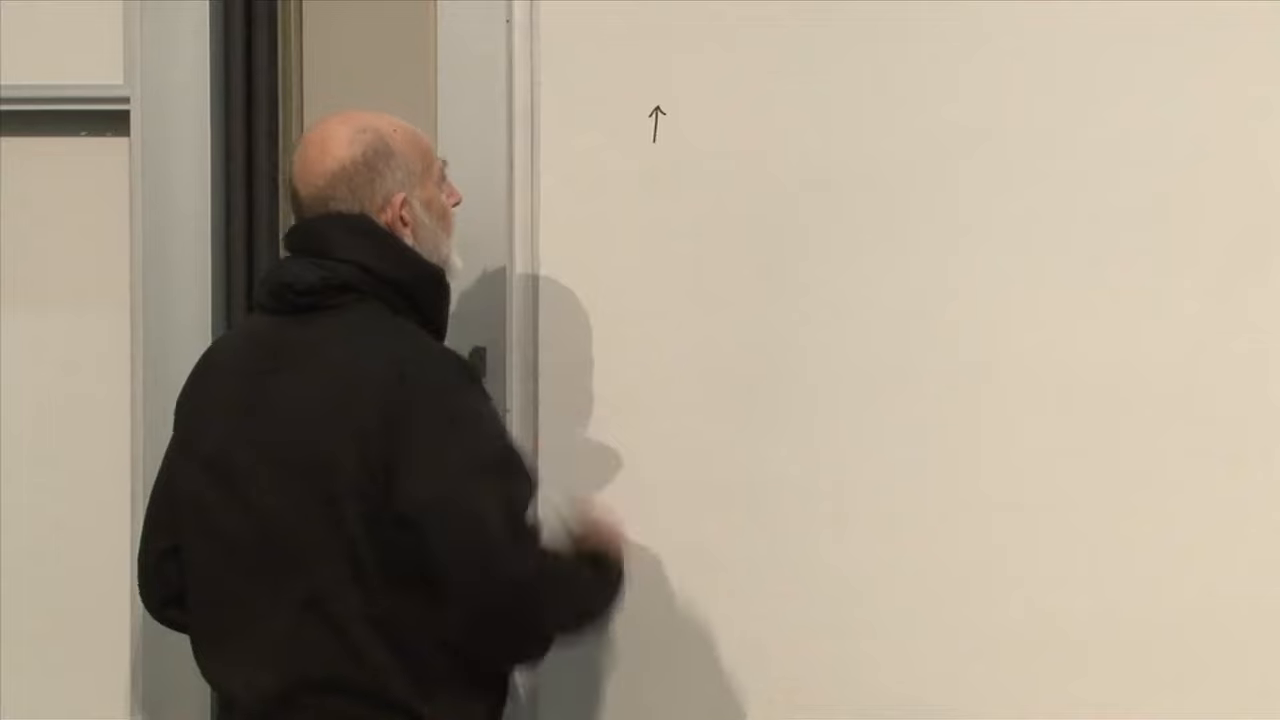
\includegraphics[width=0.64\textwidth]{lecture_02_figure_02.png}
\caption{沿某一軸製備的自旋，最初以這個記號表示。箭頭標示的是製備方式，還不是態的經典模型。}
\lectureframe{00:05:15}
\end{figure}

選擇座標軸，使\(z\)指向板上方，\(x\)指向右方，\(y\)指向板外。若儀器沿單位方向\(\hat m\)取向，測量結果為
\begin{equation}
\sigma_{\hat m}=\pm1.
\end{equation}
特別是，
\[
\sigma_z=\pm1,\qquad \sigma_x=\pm1,\qquad \sigma_y=\pm1.
\]
在這個階段，「\emph{分量}」一詞是操作性的：儀器沿\(z\)方向取向時，所報告的\(\sigma_z\)就是這個方向的測量結果。它還不是某個隱藏經典箭頭的\(z\)分量。

\subsection{可重複性與擾動}

假設一次\(z\)測量得到\(+1\)。若中間沒有任何操作，第二次\(z\)測量仍會得到\(+1\)，之後重複測量也一樣。第一次測量已將系統製備成一個態，使同一個問題有確定的答案。

\begin{classroomqa}
\audiencequestion{如果量子測量會擾動自旋，為什麼立即重複測量會得到相同結果？}
\lecturerresponse{擾動並非毫無區別。測量\(\sigma_z\)可能改變之後進行\(x\)或\(y\)測量時的結果，但新測得的\(\sigma_z\)值仍可重複取得。有用的實驗恰好需要這種有限程度的穩定性。}
\end{classroomqa}

現在將儀器轉過\(180^\circ\)。自旋在儀器朝上取向時測得\(+1\)，而儀器倒轉後則測得\(-1\)。再將儀器轉回朝上，結果又是\(+1\)。因此，儀器的取向很重要。溫度計不會因為上下顛倒就測出負溫度；自旋分析器的行為不同，因為它測量的是一個有方向性的量。

\begin{figure}[htbp]
\centering
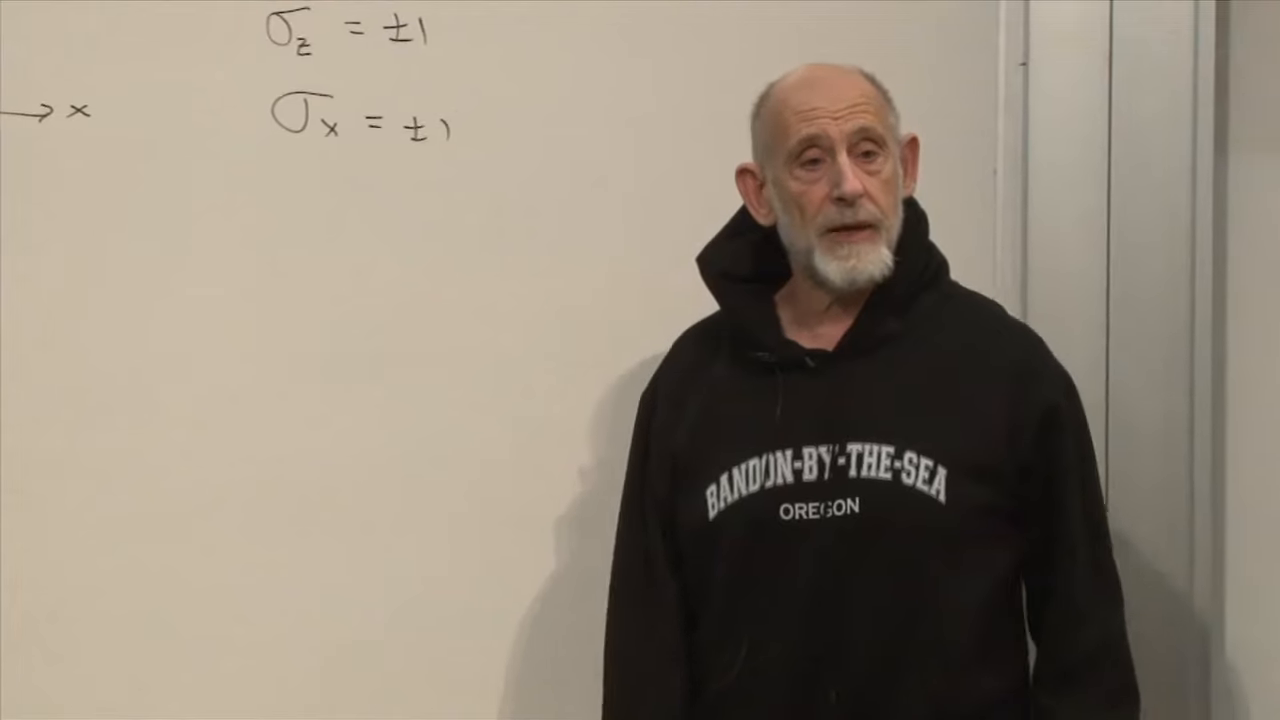
\includegraphics[width=0.72\textwidth]{lecture_02_figure_03.png}
\caption{板上記錄了二值標記\(\sigma_z=\pm1\)和\(\sigma_x=\pm1\)，以及\(x\)軸的方向提示。}
\lectureframe{00:12:46}
\end{figure}

與經典單位向量的差異立刻可見。經典分量會在\(-1\)與\(+1\)之間連續變化。垂直於\(x\)軸的單位向量，其\(x\)分量為零。相較之下，沿\(x\)方向取向的自旋分析器從不顯示零；即使自旋是沿\(z\)方向製備的，它顯示的仍是\(+1\)或\(-1\)。

\section{單次測量結果與向量式平均值}

先製備自旋，使測量得到\(\sigma_z=+1\)，然後測量\(\sigma_x\)。在以相同方式製備的試驗中，一半得到\(+1\)，另一半得到\(-1\)。因此
\begin{equation}
\langle \sigma_x\rangle=0.
\end{equation}
同樣的製備方式也得到
\begin{equation}
\langle \sigma_y\rangle=0.
\end{equation}
反過來說，以\(\sigma_x=+1\)製備的自旋，接著測量\(z\)或\(y\)時，兩種結果出現的機率相等。

這段敘述包含兩種不同的實驗。對\emph{同一個}自旋，在第一次測得\(x\)結果後反覆測量\(\sigma_x\)，只會確認該結果。要得到五五--分的統計結果，必須準備許多個處於相同\(z\)態的自旋，或讓同一個自旋在每次\(x\)測量前都重新回到相同的製備狀態。

\begin{classroomqa}
\audiencequestion{如果自旋進入儀器前沒有經過刻意製備，會發生什麼事？}
\lecturerresponse{測量結果仍是\(+1\)或\(-1\)，但各自出現的機率取決於自旋實際處於什麼態。製備是讓重複試驗具有可比性的受控程序。若兩次測量之間發生未知操作，就不能再保證結果可重複；若期間沒有任何操作，同一分量的測量結果便可重現。}
\end{classroomqa}

\subsection{任意兩個方向}

將自旋製備在單位方向\(\hat n\)上，方法是用沿\(\hat n\)方向取向的分析器測得\(+1\)。接著沿另一個單位方向\(\hat m\)測量。每次試驗的結果仍只有\(\pm1\)，但對相同製備的多次試驗取平均，得到
\begin{equation}
\boxed{\langle\sigma_{\hat m}\rangle=\hat n\cdot\hat m
=\cos\theta_{nm}.}
\label{eq:spin-average}
\end{equation}
板書將其簡寫為\(\langle\sigma_m\rangle=n\cdot m\)：

\begin{figure}[htbp]
\centering
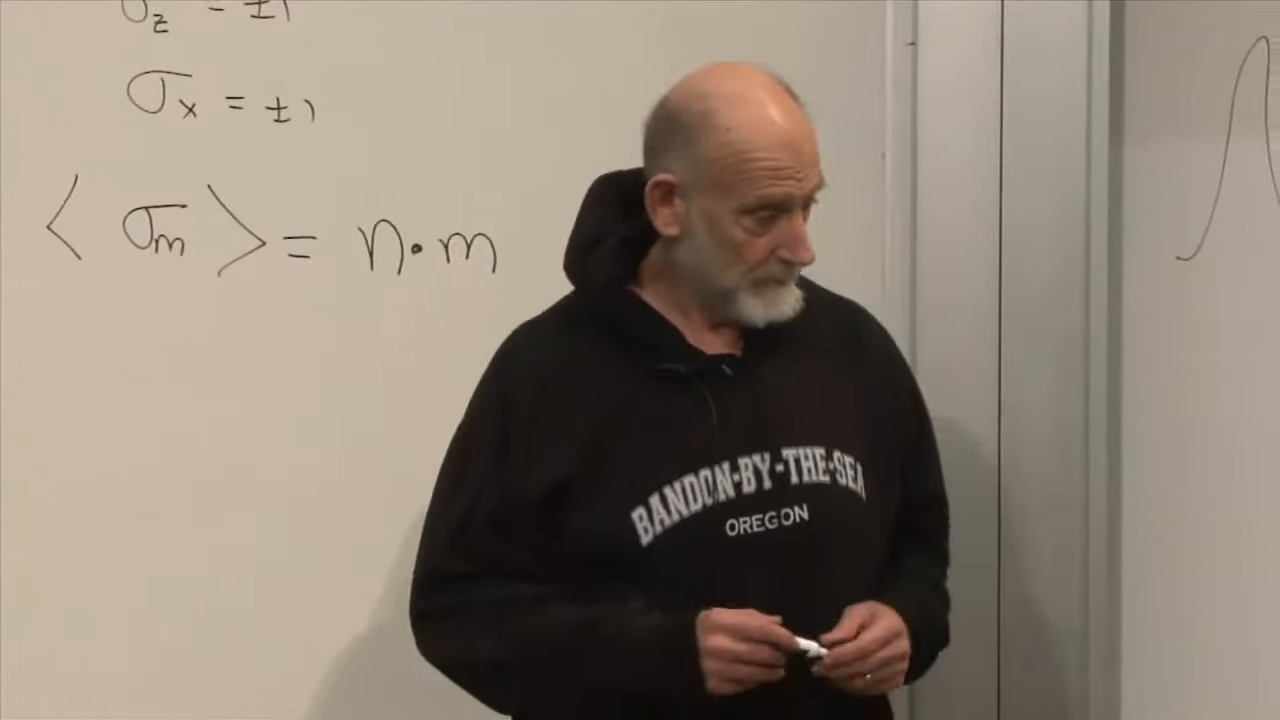
\includegraphics[width=0.74\textwidth]{lecture_02_figure_04.png}
\caption{向量式的規律適用於系綜平均值，而非單次\(\pm1\)測量結果。}
\lectureframe{00:23:22}
\end{figure}

式~\eqref{eq:spin-average}涵蓋了前述情況。若\(\hat m=\hat n\)，平均值就是\(+1\)；由於測量結果不可能大於\(+1\)，每次試驗都必定得到\(+1\)。若\(\hat m=-\hat n\)，每次試驗都得到\(-1\)。兩軸互相垂直時，平均值為零，兩種結果出現的頻率相等。

若\(p_+\)和\(p_-\)分別表示兩種可能結果的機率，則
\[
p_++p_-=1,\qquad p_+-p_-=\hat n\cdot\hat m.
\]
因此，
\begin{equation}
p_\pm=\frac{1\pm\hat n\cdot\hat m}{2}.
\label{eq:direction-probabilities}
\end{equation}
\editorialnote{講課中給出了兩種測量結果及其平均值。式~\eqref{eq:direction-probabilities}可直接由這兩項事實代數推得。}

\begin{classroomqa}
\audiencequestion{尖括號中的量是\emph{期望值}，還是一般的平均值？}
\lecturerresponse{它是多次重複測量所記錄結果的平均值。\emph{期望值}是標準術語，但這裡並沒有指另一種額外的平均方式。儀器產生一串\(+1\)和\(-1\)的結果；尖括號表示在大量試驗的極限下，這串結果的算術平均。}
\end{classroomqa}

\begin{classroomqa}
\audiencequestion{在得知平均值規律之前，箭頭\(\hat n\)是否已經具有幾何意義？}
\lecturerresponse{一開始，箭頭只是標示製備儀器的取向。反轉實驗，以及平均值對\(\hat n\cdot\hat m\)的依賴，才賦予這個標記操作上的幾何意義。分量的意義由儀器界定；單次測量結果並不對應於經典投影。}
\end{classroomqa}

這是方向圖像與離散測量資料之間的第一個調和。單個自旋的行為不像具有連續分量值的經典箭頭。然而，許多個以相同方式製備的自旋，其統計結果會如同單位三維向量的分量般變換。

\section{以集合表示經典命題}

在建構量子態空間之前，先來看經典系統中的邏輯如何運作。令可能的狀態構成集合\(\Omega\)。命題\(A\)以其中使\(A\)為真的狀態所組成的子集表示。

對於六面骰子，
\[
A=\{2,4,6\}
\]
可以表示\emph{結果為偶數}；而
\[
B=\{4,5,6\}
\]
可以表示\emph{結果大於三}。邏輯運算便對應到集合運算：
\begin{equation}
\neg A=A^c,\qquad
A\land B=A\cap B,\qquad
A\lor B=A\cup B.
\label{eq:classical-logic}
\end{equation}
此處的\(\lor\)表示包含「或」：只要\(A\)或\(B\)其中之一為真，或兩者皆真，\(A\lor B\)便為真。這不是日常用語中表示「\emph{非此即彼：\(A\)或\(B\)，但不能兩者皆是}」的排他性用法。

\begin{classroomqa}
\audiencequestion{自旋測量只有兩種結果，但製備方向可以連續變化。可能的態是有限個，還是連續無窮多個？}
\lecturerresponse{可能的製備方向構成連續集合，儘管每個選定的分析器都只有兩種讀數。這正是為什麼光靠計算探測器標記的數目，不足以描述態空間。}
\end{classroomqa}

對經典子集而言，交集與聯集不受命題提及順序影響：
\[
A\cap B=B\cap A,\qquad A\cup B=B\cup A.
\]
因此，對經典複合命題進行實驗檢驗時，可以理想化地不讓順序成為邏輯的一部分。

\section{依順序而異的「或」檢驗}

考慮以下量子命題：
\begin{equation}
A:\sigma_z=+1,\qquad B:\sigma_x=+1.
\end{equation}
每個命題都有明確的檢驗方式：將儀器沿\(z\)方向取向以檢驗\(A\)，或沿\(x\)方向取向以檢驗\(B\)。問題出在試圖檢驗\(A\lor B\)時：先檢驗其中一個命題，若結果為假，再檢驗另一個。

設想有一位看不見的製備者提供了一個\(z\)方向自旋向上的態。若先檢驗\(A\)，結果必定是\(+1\)，因此「或」檢驗的結果為\emph{真}。

若反過來檢驗，先測試\(B\)會得到
\[
P(B)=\frac12,\qquad P(\neg B)=\frac12.
\]
若\(B\)為假，這次\(x\)測量仍然會將自旋製備成一個確定的\(x\)態。接著在此態上檢驗\(A\)，結果為
\[
P(A\mid \neg B)=\frac12,\qquad
P(\neg A\mid \neg B)=\frac12.
\]
因此，反向順序的程序以機率
\begin{equation}
P(\neg B\ \text{then}\ \neg A)
=\frac12\cdot\frac12=\frac14.
\end{equation}
得到兩個命題皆為假的結果。一種順序總是判定「或」為真；另一種則有四分之一的試驗判定它為假。

\begin{classroomqa}
\audiencequestion{這個矛盾是否只是因為我們不了解那個秘密製備態？}
\lecturerresponse{不是。選擇這個隱藏的初始製備，只是為了讓比較更清楚。第一次\(x\)測量會在物理上將系統製備成一個\(x\)態，因此之後的\(z\)檢驗所測量的已是改變後的態。即使觀察者更了解初始製備，也無法消除這項干預。}
\end{classroomqa}

\begin{classroomqa}
\audiencequestion{能否改用更複雜的問題層級來檢驗「或」，而不採用這種依序檢驗的規則？}
\lecturerresponse{當然可以定義不同的實驗程序，但它們就會是不同的量子測量。不存在一個與實驗程序無關的子集\(A\cup B\)，使其真值能不受儀器影響地直接揭示。順序依賴提醒我們，經典集合邏輯並不是這些命題本身所遵循的邏輯。}
\end{classroomqa}

稍後會以投影算符表示命題。代數上的簡要警示是
\begin{equation}
P_A P_B\ne P_B P_A.
\end{equation}
目前還不需要更多運算元理論。關鍵在於，不相容的檢驗彼此不對易，因此其複合命題不能視為普通的集合聯集。

\begin{classroomqa}
\audiencequestion{能否安排這個實驗的雙粒子版本，讓檢驗方式的選擇對過去產生作用？}
\lecturerresponse{這個問題需要本章尚未介紹的理論工具。單自旋的測量序列無法導出任何反向因果的結論，因此這個問題暫且保留，不妄加猜測。}
\end{classroomqa}

\section{線性態空間}

集合包含元素，但一般沒有自然的運算能將兩個元素相加而得到第三個。線性向量空間則具有更多結構。若\(\ket{A}\)和\(\ket{B}\)是向量，且\(\alpha,\beta\in\mathbb C\)，那麼
\begin{equation}
\alpha\ket{A}+\beta\ket{B}
\end{equation}
也是同一空間中的向量。量子態以這樣的複線性空間中的向量表示。

每個右矢\(\ket{A}\)都有一個對應的對偶左矢\(\bra{A}\)。將左矢與右矢配對會得到一個複數，稱為內積。內積滿足共軛對稱性：
\begin{equation}
\braket{A}{B}=\braket{B}{A}^{*}.
\label{eq:conjugate-symmetry}
\end{equation}

\begin{figure}[htbp]
\centering
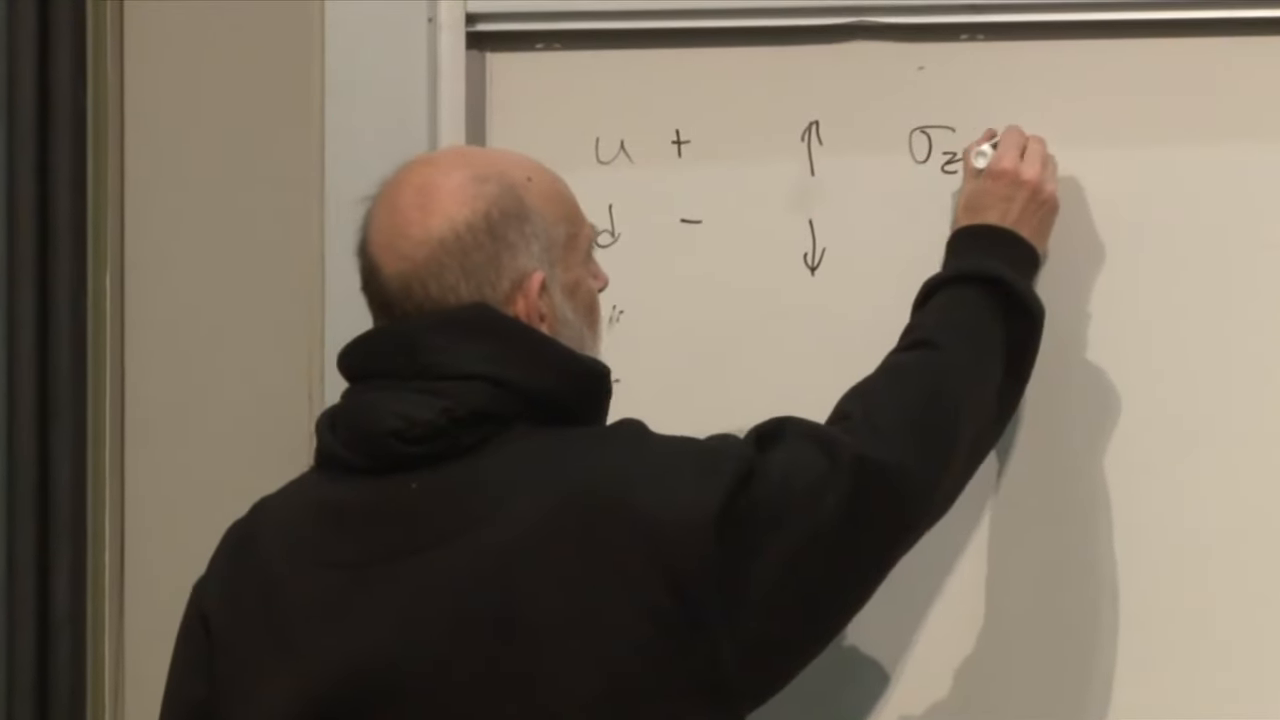
\includegraphics[width=0.78\textwidth]{lecture_02_figure_05.png}
\caption{板書總結了線性組合，以及內積在共軛下的對稱關係。}
\lectureframe{00:46:53}
\end{figure}

向量的長度平方為
\begin{equation}
\|\ket{A}\|^2=\braket{A}{A}.
\end{equation}
由式~\eqref{eq:conjugate-symmetry}可知，這個數等於其複共軛，因此是實數；內積公理也保證它非負。若
\begin{equation}
\braket{A}{B}=0.
\end{equation}
則兩個向量正交。空間的維數，是所能選取的相互正交非零方向的最大數目。

\begin{classroomqa}
\audiencequestion{每一組基底都必須由相互正交的向量組成嗎？}
\lecturerresponse{不必。基底只需線性獨立並張成整個空間。正交基底特別方便，因為容易求出係數與機率。在二維空間中，兩個不平行的向量即使內積不為零，也可以構成一組基底。}
\end{classroomqa}

\section{二維自旋空間}

假設單一自旋的態空間是二維複向量空間：
\begin{equation}
\mathcal H_{\mathrm{spin}}\cong\mathbb C^2.
\end{equation}
可能的態向量有連續無窮多個，但只需兩個線性獨立的基底向量，就能表示其中任何一個。

先從由沿\(z\)方向取向的儀器所製備的態開始：
\begin{align}
\ket{u}&\longleftrightarrow \sigma_z=+1,\\
\ket{d}&\longleftrightarrow \sigma_z=-1.
\end{align}
字母\(u,d\)、正負號\(+,-\)和箭頭\(\uparrow,\downarrow\)，都是這兩種製備方式的不同標記。由於\(z\)測量能確定地區分兩者，對應的態向量彼此正交：
\begin{equation}
\braket{u}{d}=0.
\end{equation}
並將它們的長度選為單位長度：
\[
\braket{u}{u}=\braket{d}{d}=1.
\]

於是，每個自旋態都可以寫成
\begin{equation}
\ket{A}=\alpha_u\ket{u}+\alpha_d\ket{d},
\qquad \alpha_u,\alpha_d\in\mathbb C.
\label{eq:general-spin-state}
\end{equation}
其機率規則為
\begin{equation}
P(u|A)=|\alpha_u|^2,\qquad
P(d|A)=|\alpha_d|^2.
\label{eq:born-z}
\end{equation}
由於兩種結果必有一種發生，
\begin{equation}
|\alpha_u|^2+|\alpha_d|^2=1.
\label{eq:normalization}
\end{equation}

\begin{figure}[htbp]
\centering
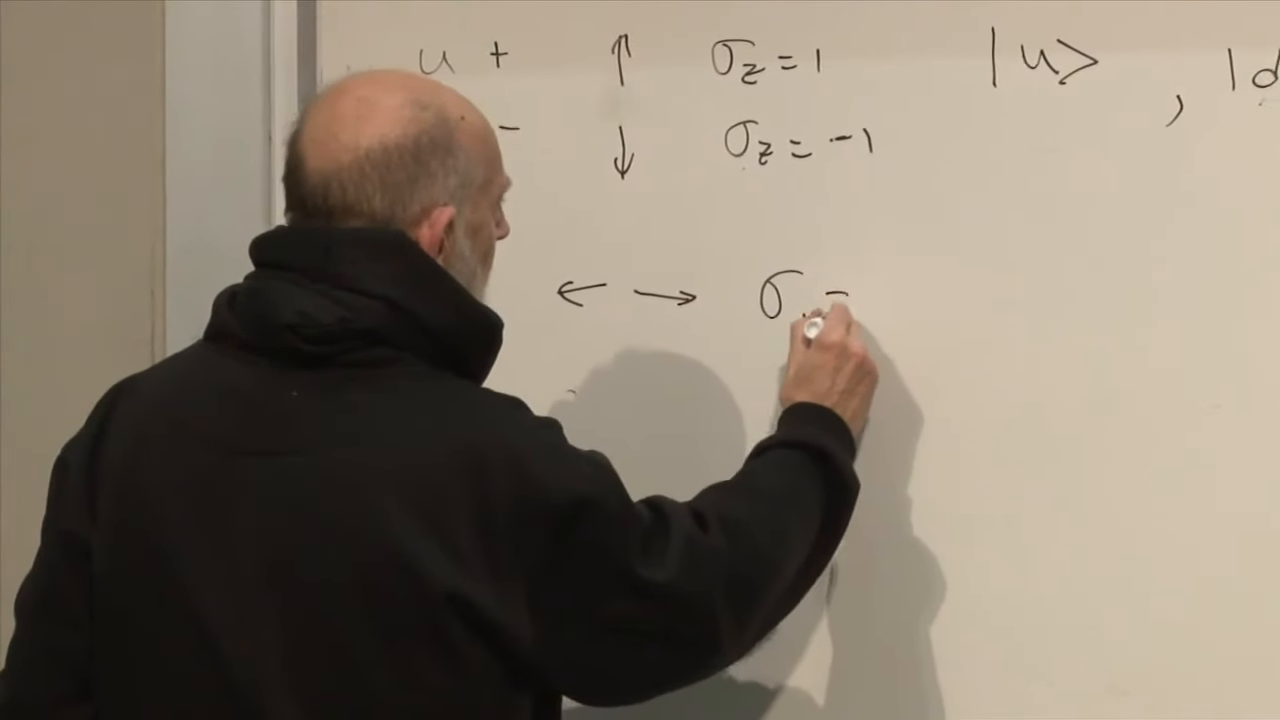
\includegraphics[width=0.78\textwidth]{lecture_02_figure_06.png}
\caption{一般的上--下態展開、兩種結果的機率總和，以及等價的單位範數條件。}
\lectureframe{01:03:38}
\end{figure}

單位範數條件可直接推出：
\begin{align}
\braket{A}{A}
&=(\alpha_u^*\bra{u}+\alpha_d^*\bra{d})
  (\alpha_u\ket{u}+\alpha_d\ket{d})\\
&=|\alpha_u|^2\braket{u}{u}
 +\alpha_u^*\alpha_d\braket{u}{d}\\
&\quad +\alpha_d^*\alpha_u\braket{d}{u}
 +|\alpha_d|^2\braket{d}{d}\\
&=|\alpha_u|^2+|\alpha_d|^2=1.
\end{align}
因此，物理純態以歸一化向量表示。

\begin{classroomqa}
\audiencequestion{這些敘述是推導出來的，還是公設？}
\lecturerresponse{目前提出的，是用來符合實驗結果的規則。二維空間、機率規則，以及正交性的詮釋，都是先以啟發式方式引入。現在可以檢查它們彼此是否一致；至於態與可觀測量之間的系統性關係，則留待接下來討論。}
\end{classroomqa}

\subsection{正交性代表可區分性}

正交性的物理意義，比把它想成箭頭互相垂直更重要：

\begin{quote}
能透過一次測量確定地區分的態，以正交向量表示。
\end{quote}

上態和下態符合這項判準。若系統處於上態，\(z\)儀器絕不會測得下態，反之亦然。若兩個態的內積非零，表示其中一個態有時可能產生與另一個態相對應的測量結果。

\section{右--左基底}

令\(\ket{r}\)和\(\ket{l}\)表示具有確定\(x\)自旋值的態：
\[
\ket{r}\longleftrightarrow\sigma_x=+1,\qquad
\ket{l}\longleftrightarrow\sigma_x=-1.
\]
由於態空間是二維的，這兩個態都必須是\(\ket{u}\)和\(\ket{d}\)的線性組合。以右向取向的儀器製備自旋時，測得上、下的機率相等，因此兩個係數的絕對值也必須相等。選用最簡單的相位約定：
\begin{equation}
\ket{r}=\frac{1}{\sqrt2}\bigl(\ket{u}+\ket{d}\bigr).
\label{eq:right-state}
\end{equation}
右態和左態可由\(x\)儀器確定地區分，因此左態必須與右態正交。一種方便的選擇是
\begin{equation}
\ket{l}=\frac{1}{\sqrt2}\bigl(\ket{u}-\ket{d}\bigr).
\label{eq:left-state}
\end{equation}
確實，
\begin{align}
\braket{l}{r}
&=\frac12(\bra{u}-\bra{d})(\ket{u}+\ket{d})\\
&=\frac12(1-1)=0.
\end{align}

\begin{figure}[htbp]
\centering
\includegraphics[width=0.82\textwidth]{lecture_02_figure_07.png}
\caption{完整的右--左態構造：上--下態的振幅大小相等、相對符號相反，且內積為零。}
\lectureframe{01:12:15}
\end{figure}

\(\ket{l}\)的整體負號只是約定。將\(\ket{l}\)改成\(-\ket{l}\)，不會改變任何測量機率。將式~\eqref{eq:right-state}與式~\eqref{eq:left-state}相加及相減，可得反向的基底變換：
\begin{align}
\ket{u}&=\frac{1}{\sqrt2}\bigl(\ket{r}+\ket{l}\bigr),\\
\ket{d}&=\frac{1}{\sqrt2}\bigl(\ket{r}-\ket{l}\bigr).
\end{align}
這種對稱性很重要。以\(x\)基底表示時，上態或下態是右態與左態的等權重疊加；同樣地，右態或左態也是上態與下態的等權重疊加。

\section{內--外基底與相對相位}

將儀器沿\(y\)方向取向，使其垂直於板面。寫成
\[
\ket{i}\longleftrightarrow\sigma_y=+1,\qquad
\ket{o}\longleftrightarrow\sigma_y=-1,
\]
其中右矢標記\(i\)表示\emph{內}；而乘在右矢前、未加其他標記的\(i\)仍表示虛數單位。

上、下結果的機率相等，要求兩個係數的絕對值相等。內態與外態正交，則要求兩者之間具有適當的相對相位，使內積為零。一種對稱的選擇是
\begin{align}
\ket{i}&=\frac{1}{\sqrt2}\bigl(\ket{u}+i\ket{d}\bigr),\\
\ket{o}&=\frac{1}{\sqrt2}\bigl(\ket{u}-i\ket{d}\bigr).
\label{eq:in-out-states}
\end{align}
在\((u,d)\)基底中，六個態為
\begin{align}
\ket{u}&=\binom10,
&
\ket{d}&=\binom01,
\\
\ket{r}&=\frac1{\sqrt2}\binom11,
&
\ket{l}&=\frac1{\sqrt2}\binom1{-1},
\\
\ket{i}&=\frac1{\sqrt2}\binom1{i},
&
\ket{o}&=\frac1{\sqrt2}\binom1{-i}.
\end{align}

\begin{figure}[htbp]
\centering
\includegraphics[width=0.82\textwidth]{lecture_02_figure_08.png}
\caption{上--下基底中的六個列向量。下面一對向量的相對虛數相位符號相反。}
\lectureframe{01:20:50}
\end{figure}

計算內積以檢查正交性時，左矢中的複共軛不可或缺：
\begin{align}
\braket{i}{o}
&=\frac12(\bra{u}-i\bra{d})(\ket{u}-i\ket{d})\\
&=\frac12\bigl(1+(-i)(-i)\bigr)=0.
\end{align}

\begin{classroomqa}
\audiencequestion{選擇以\(+i\)表示\emph{內}態，而以\emph{外}態作為另一個標記，是否編碼了空間座標軸的右手性？}
\lecturerresponse{這裡已引入一項約定；等到介紹泡利矩陣和旋轉後，其幾何意義會更加清楚。目前只需確保這一對態彼此正交，並與其他基底成對稱關係；交換標記或反轉\(y\)軸，改變的是約定，不會影響這套構造的一致性。}
\end{classroomqa}

\subsection{在右--左基底中檢查對稱性}

在內態中使用
\[
\ket{u}=\frac{\ket{r}+\ket{l}}{\sqrt2},\qquad
\ket{d}=\frac{\ket{r}-\ket{l}}{\sqrt2}
\]：
\begin{align}
\ket{i}
&=\frac1{\sqrt2}
\left(
\frac{\ket{r}+\ket{l}}{\sqrt2}
+i\frac{\ket{r}-\ket{l}}{\sqrt2}
\right)\\
&=\frac{1+i}{2}\ket{r}
 +\frac{1-i}{2}\ket{l}.
\label{eq:in-in-rl}
\end{align}
雖然兩個係數都沒有明顯出現\(1/\sqrt2\)，
\begin{equation}
\left|\frac{1+i}{2}\right|^2
=\left|\frac{1-i}{2}\right|^2
=\frac12.
\end{equation}

\begin{figure}[htbp]
\centering
\includegraphics[width=0.82\textwidth]{lecture_02_figure_09.png}
\caption{內態的基底變換，以及右--左態的機率皆為\(1/2\)的檢查。}
\lectureframe{01:29:10}
\end{figure}

因此，三組基底中任一組的每個態，在另外兩組基底中的任一組測量時，都會得到相等的機率。\(z\)、\(x\)和\(y\)基底彼此互為無偏基底。

\section{為何有三組特殊基底}

\begin{classroomqa}
\audiencequestion{是否可能存在第四對態，與這三對態之間的對稱關係相同？}
\lecturerresponse{對單一二態系統而言，不可能。一旦固定了三對互為無偏的態，就不存在具有相同等重疊關係的第四對。這三個特殊標記對應三個空間方向，與普通空間的三個維度有關，儘管複數態空間本身只有二維。}
\end{classroomqa}

這種關聯可從物理參數的計數看出。一般的列向量
\[
\binom{\alpha_u}{\alpha_d}
\]
包含兩個複數，也就是四個實數。歸一化條件去掉一個自由度：
\[
|\alpha_u|^2+|\alpha_d|^2=1.
\]
將兩個分量同乘一個整體相位，不會改變任何測量機率：
\begin{equation}
\ket{A}\sim e^{i\chi}\ket{A}.
\label{eq:global-phase}
\end{equation}
這又去掉一個實參數。因此
\begin{equation}
4-1-1=2
\end{equation}
剩下兩個物理實參數，恰好等於描述三維空間中一個方向所需的角度數目。

以下這種方便的表示法，清楚呈現了兩者的關係：
\begin{equation}
\ket{\psi(\theta,\phi)}
=\cos\frac{\theta}{2}\,\ket{u}
+e^{i\phi}\sin\frac{\theta}{2}\,\ket{d}.
\label{eq:bloch-parameterization}
\end{equation}
\editorialnote{~\eqref{eq:bloch-parameterization}是講課所指出的雙參數族之標準歸一化表示式。此處列出明確的半角形式，讓參數計數更具體；它的動力學與旋轉詮釋則留待後續課程。}

\begin{classroomqa}
\audiencequestion{忽略整體相位的精確數學意義是什麼？}
\lecturerresponse{圓周\(\{e^{i\chi}\ket{\psi}\}\)上的所有歸一化向量都代表同一個物理態。這些向量被視為等價，就像把由既定冗餘關係相連的點視為同一個物理點。分量間的相對相位仍可測量；只有乘在整個向量上的相位會被忽略。}
\end{classroomqa}

\begin{classroomqa}
\audiencequestion{計算中仍會用到未歸一化向量，或具有負分量的向量嗎？}
\lecturerresponse{會。線性代數容許這類向量，而且計算中的中間向量不必已代表一個製備好的物理態。非零向量可以在最後再歸一化。負分量與複數分量是振幅，不是負機率；態歸一化後，振幅絕對值的平方才給出機率。}
\end{classroomqa}

\begin{classroomqa}
\audiencequestion{在更高維空間或更複雜的旋量中，這套圖像會如何延伸？}
\lecturerresponse{相同的線性原理仍然適用，但態空間維數、空間旋轉與可觀測自旋之間的關係會更為豐富。這項延伸超出目前二態系統的討論範圍。}
\end{classroomqa}

\section{正交性不等於空間中的垂直}

「\emph{正交}」一詞現在具有抽象且操作性的意義，不能與普通空間中所畫兩支箭頭的夾角混淆。空間方向上的上與下互為相反方向，但態向量\(\ket{u}\)和\(\ket{d}\)彼此正交。空間方向上的上與右互相垂直，但
\begin{equation}
\braket{u}{r}=\frac1{\sqrt2}\ne0.
\end{equation}

\begin{classroomqa}
\audiencequestion{為什麼相反的空間方向所對應的態會正交，互相垂直的空間方向所對應的態卻不正交？}
\lecturerresponse{態空間中的重疊量度的是實驗上的可區分性，而非標記方向之間的歐幾里得夾角。上態與下態可透過一次\(z\)測量確定地區分，因此兩者的內積為零。上態與右態則無法如此區分：以右向製備的自旋，有時會測得上態。因此，兩個態向量之間有非零重疊。}
\end{classroomqa}

經典機率論也有類似的概念。兩個支撐集不相交的機率分布可以完全區分：觀察結果就能判定採用的是哪一個分布。支撐集相交的分布則無法只根據單次取樣而無誤差地區分。量子正交性相當於支撐集不重疊；非零內積則表示某些結果可能由兩種製備中的任一種產生。

\begin{classroomqa}
\audiencequestion{是否應把二維態空間想像成包含上向與右向箭頭的物理平面？}
\lecturerresponse{不應如此。標記\(x,y,z\)代表普通空間中儀器的取向。右矢則屬於具有自身內積的複向量空間。參數計數說明了兩種結構之間的關聯，但若把兩者的圖像逐點等同，就會混淆空間方向的垂直與態空間中的正交。}
\end{classroomqa}

\section{態、測量與接下來的問題}

到目前為止，這套構造是藉由使向量符合操作上的事實而逐步建立的。三種裝置取向標示出三對正規化態，而各態之間的重疊則重現了觀測到的機率。嚴謹的處理仍須說明，像 \(\sigma_z\) 這樣的可觀測量如何作用於態，以及為何其可能的測量結果就是它的本徵值。接下來要處理的正是這一步。

先前的邏輯謎題，現在可以更精確地表述。命題對應於子空間或其投影算符，而不相容的投影算符彼此不對易。那個對順序敏感的「或」測試並非語言上的悖論，而是這種非對易結構的早期呈現。

\begin{classroomqa}
\audiencequestion{如果態不是一般意義上的箭頭，為什麼三個標記 \(x,y,z\) 和平均值 \(\langle\sigma_{\hat m}\rangle\) 看起來如此經典？}
\lecturerresponse{經典向量會出現在系綜平均中。單一自旋給出離散的答案，而許多以相同方式製備的自旋，其平均值則會像方向向量的分量那樣變換。當大量粒子使這些平均值趨於穩定時，宏觀的經典行為便會浮現；不應反過來將此解讀為每個單一自旋都隱藏著一個連續的取值。}
\end{classroomqa}

\begin{classroomqa}
\audiencequestion{共同相位的冗餘是規範不變性的一個例子嗎？}
\lecturerresponse{這是共同相位下的一種簡單不變性，也預示了更廣泛的規範概念。在此處深入探討這項關聯，會超出目前這套構造的範圍，因此只保留與物理相關的說法：共同相位不可觀測，相對相位則可以。}
\end{classroomqa}

最後，不應把測量想成只是揭示自旋一直以經典意義攜帶著的某個值。測量會製備出與記錄結果相對應的態。因此，立即重複同一測量時，結果會前後一致；而對一組重新以相同方式製備的自旋進行測量，則會呈現由相關振幅決定的機率分佈。將可觀測量引入為算符後，便能精確描述這種製備與讀出的數學過程。